\section{Creating Language Definition in MPS}
\label{sect:LANGDEF}

The proposed INGRID method accepts grammars in the ANTLR v4 notation~\cite{ref:ANTLRBOOK} as input.
All widely used programming languages have their syntax defined using this notation~\footnote{https://github.com/antlr/grammars-v4}.
Unlike some of the related projects, we did not extend the notation with any custom features, and we also did not create an MPS language for the ANTLR notation.

The process of MPS language construction, as performed by INGRID, consists of four phases --- the first is parsing of the input grammar, which is followed by definition of the essential aspects (Structure, Editor, and TextGen).
Each of the phases 2-4 is exclusively and fully responsible for one aspect.

INGRID is currently able to create (i) a full Structure aspect for each element (type of an AST node) of the given language, (ii) a very basic Editor, and (iii) a basic TextGen aspect.
Therefore, the resulting MPS language typically still has to be adjusted manually to improve its usability, and the human users must also define the remaining aspects not yet supported by INGRID.

Our approach differs from the related projects (Section~\ref{sect:RELATED}) especially in the level of automation. It also has much better support for the definition of Editor and TextGen.

\subsection{Running Example}

We will describe the INGRID method using the example of a simplified XML language that is defined in Figure~\ref{fig:SIMPLEXML}.
The \emph{SimpleXML} language is small but complex enough to be used for illustration of the main challenges and behavior of the proposed algorithms.

\begin{figure*}[ht]
\centering
\begin{framed}
\begin{alltt}
\textbf{grammar} \textit{SimpleXML};
\antlrparserrule{document}  : \antlrparserrule{prolog}? \antlrparserrule{comment}? \antlrparserrule{element} ;
\antlrparserrule{prolog}    : \antlrliteral{<?xml } \antlrparserrule{attrib}* \antlrliteral{?>} ;
\antlrparserrule{comment}   : \antlrliteral{<!--} \antlrlexerrule{TEXT} \antlrliteral{-->} ;
\antlrparserrule{element}   : \antlrliteral{<} \antlrlexerrule{Name} \antlrparserrule{attrib}* \antlrliteral{>} \antlrparserrule{content}* \antlrliteral{</} \antlrlexerrule{Name} \antlrliteral{>} | \antlrliteral{<} \antlrlexerrule{Name} \antlrparserrule{attrib}* \antlrliteral{/>} ;
\antlrparserrule{attrib}    : \antlrlexerrule{Name} \antlrliteral{="} \antlrlexerrule{TEXT} \antlrliteral{"} ;
\antlrparserrule{content}   : \antlrlexerrule{TEXT} | \antlrparserrule{element} | \antlrparserrule{comment} | \antlrlexerrule{CDATA} ;
\antlrlexerrule{Name}      : \antlrlexerrule{NameStartChar} \antlrlexerrule{NameChar}* ;
\textbf{fragment}
\antlrlexerrule{DIGIT}     : \antlrregex{[0-9]} ;
\textbf{fragment}
\antlrlexerrule{NameChar}  : \antlrlexerrule{NameStartChar} | \antlrliteral{-} | \antlrliteral{\_} | \antlrliteral{.} | \antlrlexerrule{DIGIT} ;
\textbf{fragment}
\antlrlexerrule{NameStartChar} : \antlrregex{[:a-zA-Z]} ;
\antlrlexerrule{TEXT}      : \antlrregex{~[<"]*} ;
\antlrlexerrule{CDATA}     : \antlrliteral{<![CDATA[} \antlrregex{.*?} \antlrliteral{]]>} ;
\end{alltt}
\end{framed}
\caption{Grammar of the SimpleXML language in the ANTLR v4 notation}
\label{fig:SIMPLEXML}
\end{figure*}

The grammar of SimpleXML contains elements of the kinds that are listed below.
Each color in Figure~\ref{fig:SIMPLEXML} corresponds to a different kind in a way that is indicated by the list item headers.
\begin{itemize}
	\item \textbf{ANTLR v4 keywords} are required by the notation.
	\item \antlrparserrule{\textbf{Parser rules}} describe the structure of a language.
		Alternatives on the right side of a rule are separated by the pipe character ($|$).
	\item \antlrlexerrule{\textbf{Lexer rules}} describe terminal symbols that the parser matches against the input string.
		A terminal symbol can be encoded as a string value or using a regular expression.
		The \textbf{fragment} keyword states that the lexer rule just brings more clarity into the notation but it is not visible in the parser output.
	\item \antlrliteralnoap{\textbf{String literals}}, always written inside of a pair of single quote marks, also represent terminal symbols, but by exact match to a string constant.
	\item \antlrregex{\textbf{Regular expressions}} describe string tokens to be matched against regular expressions with a special ANTLR v4 regex notation\footnote{https://github.com/antlr/antlr4/blob/master/doc/lexer-rules.md}.
\end{itemize}
Elements on the right side of a rule can be annotated with standard EBNF operators (\code{?}, \code{+}, \code{*}) that specify the allowed number of occurrences.

\subsection{Parsing Input Grammar}

The first phase in the process of MPS language construction is parsing of the input grammar that is defined using the ANTLR v4 notation.
An output of this phase is an AST representing the grammar.
Nodes of the AST correspond to rules and other grammar elements.

Nevertheless, the full AST, which comes out of the automatically generated parser, is quite complex and contains information not relevant for the INGRID algorithm.
In order to get a simple representation that is easy process by the later phases and keeps only information necessary for the construction of MPS languages, several steps of post-processing of the AST have to be performed in this phase.

A simplified tree of objects is derived from the AST in two passes over the grammar.
The result of the first pass is a tree where each node contains names of other referenced rules in the form of strings.
In the second pass, the whole tree is traversed and all the references are resolved to have a form of real pointers to other rule objects.

The representation of lexer rules (tokens) in the AST has to be simplified too.
Note that, in the ANTLR notation, lexer rules can be built from alternatives just like the parser rules --- see, for example, the lexer rule \antlrlexerrule{Name} from our SimpleXML language (Figure~\ref{fig:SIMPLEXML}).
For each lexer rule, the parser produces a tree that captures the structure of the rule.
However, the lexer rules are, in fact, just regular expressions used to recognize tokens in the input string.

Every tree that represents a lexer rule is flattened into the equivalent regular expression by the recursive algorithm specified in Figure~\ref{fig:ALGFLATTEN}.
A distinct sequence is created from the elements of each alternative, and then all those sequences are joined by the alternation operator \code{$|$} to form a regular expression.

\begin{figure}[ht]
\centering
\begin{framed}
\begin{alltt}
Flatten(\textit{R}):
  \textit{T} = empty list
  \textbf{for each} alternative \textit{A} \textbf{in} rule \textit{R}:
    \textit{R} = \antlrap\antlrap
    \textbf{for each} element \textit{E} \textbf{of} \textit{A}:
      \textbf{if} \textit{E} is not yet flattened \textbf{then}:
        Flatten(\textit{E})
      \textit{R}.append(\textit{E})
      \textit{R}.append(\textit{E}.operator)
    \textit{T}.add(\textit{R})
  build string S from elements of \textit{T}:
    \textit{S} = \(t\sb{1}\) | \(t\sb{2}\) | \(\ldots\) | \(t\sb{n}\)
  \textbf{return} \textit{S}
\end{alltt}
\end{framed}
\caption{Flattening algorithm}
\label{fig:ALGFLATTEN}
\end{figure}

The output of \texttt{Flatten(Name)}, i.e. application of the algorithm to the \antlrlexerrule{Name} rule, is this regular expression:

\begin{center}
  \texttt{[:a-zA-Z]([:a-zA-Z]|\textbackslash-|{\_}|\textbackslash.|[0-9])*}
\end{center}
It defines the syntactically valid identifiers of elements and attributes in SimpleXML.
Each identifier must begin with a letter, followed by any combination of letters, digits, underscore, dash, or a dot.






% TODO continue from here



\subsection{Structure}

\todo{We import/generate the complete/full language structure fully automatically.}

Now, as the next step, we need to translate/transform the AST (the types of AST nodes) derived from the input grammar into elements of the structure aspect of the MPS language definition (into types of AST nodes), and linking the nodes appropriately.

The goal of this second step is to translate (transfer) the syntax (structure) of the input language that is captured by the grammar (ANTLR), into the MPS structure aspect.
The structure of the MPS language is somewhat similar to the grammar.
This is (the part) where INGRID spares the user from many hours of tedious and sometimes quite challenging work.
The process of transferring grammar rules into the structure of a MPS language presents/involves some interesting challenges.

As we already indicated in the introduction, the main problem/difficulty/challenge related to Structure (creating the structure) is that a grammar typically contains many rules that do not directly correspond to AST nodes and programming language constructs.
Challenges/issues related to input grammars --- intermediate rules in the syntax hierarchy that allow humans to understand the grammar better (structure aspect/component).
There is a challenge/issue that is related to construction of the structure aspect.
Grammars are written by humans and therefore contain some structures (intermediary layers) inside of them that help a human brain to understand it better.
However, these structures add unnecessary levels to its syntax hierarchy which lead to problems when using this language inside MPS.
The input grammar (EBNF, ANTLR) serves a little bit different purpose than MPS language, and the way grammar rules are usually written down causes some problems that we had to overcome in order to recreate the language inside MPS.
Note that the challenges and problems are not specific to MPS --- they are common for everyone tackling a similar problem.
In the rest of this section, we describe our solution to this problem/challenge.

We are going to describe two different approaches that we designed --- the straightforward approach (Section~\ref{sect:straightforward_approach}) and the shortcut approach (Section~\ref{sect:shortcut_approach}).
We will describe two possible approaches that we developed in Section X and Section Y, respectively.
\todo{Rict neco jako ze ten druhy, slozitejsi, approach vlastne rozsiruje ten prvni, jednodussi.}

However, before focusing on the two approaches, we must describe the basic principles of translation from the AST representing the grammar to the MPS structure, which are common to both approaches.
The structure is created according to object-oriented principles.
Each node (element) is represented by an object (and can be treated as such) that may have a parent node, child nodes, and properties of any data type (similar to fields), it may implement any number of interfaces, and it may also hold references to other nodes.
For every rule of the grammar (for every node in the grammar AST) that breaks into more/multiple alternatives, we must create a node in the MPS structure AST for each alternative of the grammar (every child node).
Names of the nodes for alternatives are composed from the name of the rule and a number indicating the order of appearance in the grammar.
For example, consider the fragment of the grammar of the SimpleXML language in Figure~\ref{fig:xmlelementrule}.
Results of this step for the first alternative, which represents the represents the full XML tag with content, can be seen in Figure~\ref{fig:element_node_common}.

\begin{figure*}[ht]
\centering
\begin{framed}
\begin{alltt}
	\antlrparserrule{element} : \antlrliteral{<} \antlrlexerrule{Name} \antlrparserrule{attrib}* \antlrliteral{>} \antlrparserrule{content}* \antlrliteral{</} \antlrlexerrule{Name} \antlrliteral{>} | \antlrap<\antlrap Name attrib* \antlrap/>\antlrap ;
\end{alltt}
\end{framed}
\caption{Element rule from the SimpleXML grammar}
\label{fig:xmlelementrule}
\end{figure*}

\begin{figure}[ht]
	\centering
	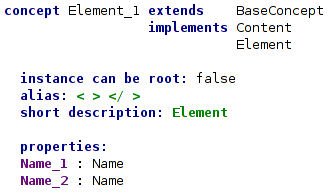
\includegraphics[scale=0.75]{./images/element_node_common.png}
	\caption{Resulting Element{\_}1 node}
	\label{fig:element_node_common}
\end{figure}

String literals (e.g., keywords such as \textbf{for}) are omitted/skipped because they will appear only in the corresponding projectional editor.
The node named \mpsconcept{Element{\_}1} contains two properties, one for each reference to the lexer rule \antlrlexerrule{Name} inside the first alternative of the \antlrparserrule{element} rule,
Value of the property will be restricted using the regular expression representing the \antlrlexerrule{Name} rule.
We explain later how the references to parser rules (\antlrparserrule{attribute} and \antlrparserrule{content}) as this is where the approaches differ.
The main/key difference between these two lies in the way we create children fields for parser rules and in the way we are going to link them together using interface concepts.

\subsubsection{The Straightforward Approach}
\label{sect:straightforward_approach}

The key idea of this approach is that, for each rule with more than one alternative, an interface node is created.
Consider the \antlrparserrule{content} rule from our SimpleXML language (Figure~\ref{fig:contentrule}).

\begin{figure}[ht]
\centering
\begin{framed}
\begin{alltt}
	\antlrparserrule{content}    :   \antlrlexerrule{TEXT}
           |   \antlrparserrule{element}
           |   \antlrparserrule{comment}
           |   \antlrlexerrule{CDATA}
           ;
\end{alltt}
\end{framed}
\caption{Content rule}
\label{fig:contentrule}
\end{figure}

Any of the four nodes corresponding to alternatives could appear anywhere the \antlrparserrule{content} rule is referenced.
So we will create one interface node, and then for each alternative of this rule we create one node that implements the interface.
The resulting fragment of structure will look like the one in Figure~\ref{fig:icontentitf}.

\begin{figure}[ht]
\centering
\begin{framed}
\begin{alltt}
	\mpsinterface{IContent}   :   \mpsconcept{Content{\_}1}
           |   \mpsconcept{Content{\_}2}
           |   \mpsconcept{Content{\_}3}
           |   \mpsconcept{Content{\_}4}
\end{alltt}
\end{framed}
\caption{IContent interface}
\label{fig:icontentitf}
\end{figure}

References to other parser rules are captured by links to children (interfaces or object nodes) in the AST nodes.
For the \antlrparserrule{element} rule that is referencing the \antlrparserrule{content} rule, defined as in Figure~\ref{fig:xmlelementrule}, we get the AST node representing the first alternative that is shown in Figure~\ref{fig:element_node_full}.
There is one \mpsinterface{IElement} interface node that is implemented by two object nodes \mpsconcept{Element{\_}1}, \mpsconcept{Element{\_}2}.
The node \mpsconcept{Element{\_}1} has two child links pointing to \mpsinterface{IAttribute} and \mpsinterface{IContent}.

\begin{figure}[ht]
	\centering
	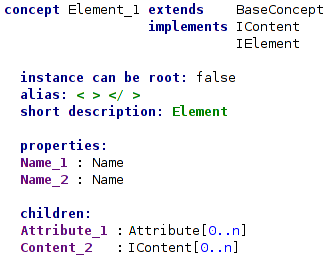
\includegraphics[scale=0.75]{./images/element_node_full.png}
	\caption{Element{\_}1 node's structure aspect}
	\label{fig:element_node_full}
\end{figure}

A problem with this approach, which we call \emph{the layer problem}, is related to the grammar rules (and corresponding AST nodes) that represent intermediary layers created only to make the grammar more readable.
The intermediary layers are created by authors of the grammars in order to make them more readable and more easily (better) maintainable.
We illustrate this problem (and explain it) on the behavior of auto-completion in MPS.
Imagine there is a freshly inserted \mpsconcept{Element{\_}1} node (representing the full XML element as is stated in the first alternative of the \antlrparserrule{element} parser rule).
Now we would like to insert another nested XML element inside.
MPS auto-completion mechanism would give us four options that are captured in the left part of Figure~\ref{fig:layer_problem}.
This is because there exist four nodes (objects) that implement the \mpsinterface{IContent} interface as per each alternative of the rule.

\begin{figure*}[ht]
	\centering
	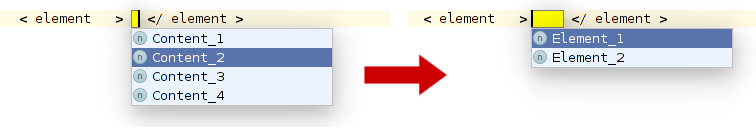
\includegraphics[scale=0.5]{./images/layer_problem.png}
	\caption{Layer problem in auto-completion}
	\label{fig:layer_problem}
\end{figure*}

However, in order to correctly insert another nested element inside, a user would have to first insert the \mpsconcept{Content{\_}2} node inside \mpsconcept{Element{\_}1} that has an \mpsinterface{IElement} child inside (and nothing else).
Then, as the second step, a user would invoke/trigger/call for the auto-complete again and insert either \mpsconcept{Element{\_}1} or \mpsconcept{Element{\_}2} inside \mpsconcept{Content{\_}2}.
This mean that a user would have to go through two steps, and in the first stepe either correctly guess (or remember the grammar rule's alternative order), which option/item offered by the auto-complete menu to select.

Similarly, if one would decide to replace the nested \mpsconcept{Element{\_}1} node with, let's say, an XML comment (a \mpsconcept{Comment} node), we need to delete both intermediary layers before we get back to the original \mpsconcept{Content{\_}X} selection (crossroads).
The user cannot really see what is happening, since the intermediary level has no appearance or indicator.
This may lead to confusion on the user's part.

The layer problem is solved/addressed by the second approach, which we describe in the next subsection.

\subsubsection{The Shortcut Approach}
\label{sect:shortcut_approach}

The key idea of this approach is to identify rules and nodes that are at the end of the (derivation, inheritance) chain, and offer them directly to the user through the auto-completion menu.
We call such \emph{end rules} and \emph{end nodes}, respectively, because they cannot transparently break into more rules/nodes.

\begin{figure*}[ht]
\centering
\begin{framed}
\begin{alltt}
	\antlrparserrule{content} : \antlrlexerrule{TEXT} | \antlrparserrule{element} | \antlrparserrule{comment} | \antlrlexerrule{CDATA} ;
	\antlrparserrule{element} : \antlrliteral{<} \antlrlexerrule{Name} \antlrparserrule{attrib}* \antlrliteral{>} \antlrparserrule{content}* \antlrliteral{</} \antlrlexerrule{Name} \antlrliteral{>} | \antlrliteral{<} \antlrlexerrule{Name} \antlrparserrule{attrib}* \antlrliteral{/>} ;
	\antlrparserrule{comment} : \antlrliteral{<!--} \antlrlexerrule{TEXT} \antlrliteral{-->} ;
\end{alltt}
\end{framed}
\caption{Content parser rule with children}
\label{fig:contentrulewithchildren}
\end{figure*}

For example, the \antlrparserrule{content} rule, given in Figure~\ref{fig:contentrulewithchildren} together with its child rules, can ultimately expand into following nodes:

\begin{itemize}
	\itemsep0em
	\item \textbf{Content{\_}1} (TEXT)
	\item Content{\_}2 $\rightarrow$ \textbf{Element{\_}1}
	\item Content{\_}2 $\rightarrow$ \textbf{Element{\_}2}
	\item Content{\_}3 $\rightarrow$ \textbf{Comment}
	\item \textbf{Content{\_}4} (CDATA)
\end{itemize}

The end nodes are highlighted using the bold font.

Figure XY shows the algorithm (in pseudocode) that finds all end rules for a given parser rule.

% TODO pouzit standardni environment pro algoritmy
\begin{figure*}[ht]
\centering
\begin{framed}
\begin{alltt}
	FindPathsToEndNodes($R$):
	  Define $L$ as an empty list of list of nodes
	  Return FindPathsToEndNodes($R$, $L$)

	FindPathsToEndNodes($R$, $L$):
	  Define $Q$ as list of list of nodes
	  For each alternative $A$ of rule $R$:
	    $L1$ = Clone($L$)
	    If $A$ is a parser rule with only one element $E$:
	      Let $I$ be interface/concept representing rule $E$
	      $L1$.Add($I$)
	      $P$ = FindPathsToEndNodes($E$, $L1$)
	      $Q$ = Merge($Q$, $P$)
	    Else
	      $L1$.Add($R$)
	      Let $P$ be concept representing $A$
	      $L1$.Add($P$)
	      $Q$.Add($L1$)
	  Return $Q$
\end{alltt}
\end{framed}
\caption{Algorithm for finding end rules}
\label{fig:shortcut_algorithm}
\end{figure*}

To find end rules for each parser rule, the algorithm recursively scans through the parser tree that was built before.
For each parser rule, it tries to find paths leading to some end rule through its alternatives:
\begin{itemize}
	\item Whenever it finds an alternative that contains only one element, and this element is a reference to another parser rule, it has found an intermediary level that can be transparently hidden from the user of the language.
		The process (algorithm) continues by recursively processing alternatives of this "level" rule (since we are not at the end of the chain yet).
	\item Otherwise, an end rule was found (recursion stops here).
\end{itemize}

By appending the rule that is leading to current element (line 12) and then appending that alternative's element itself (line 14), we get a path that contains the full path and the target end rule as the last element of the chain.
The result of this algorithm, for example for the \antlrparserrule{content} rule, equals the listing of the five paths mentioned above.

We do/repeat this for all parser rules and for each rule we get a list of paths that lead from that particular rule to an end node.
We call these paths as \textbf{shortcuts}, because they provide a shortcut from the rule to the end of the chain.
Now that we have the shortcuts, we will discuss several ways how to use the shortcuts (them) to improve the MPS language under construction (how to make the language better).

The primary use of shortcuts is to generate options for the auto-completion menus such that only the end nodes are offered.
This can be technically done in two ways --- (1) through custom auto-complete menus and deletion handlers or (2) by defining a special interface for each rule such that the interface is implemented only by end nodes for the rule.
Shortcuts have to be considered when inserting nodes but also when deleting them, i.e. the whole chain (shortcut path) consisting of possibly multiple intermediary AST nodes (levels) up to the end node must be added, respectively deleted.
The effect of insertion must be fully reversed when the user wants to delete some end node (the given end node).

\subsection{Editor}

\todo{Definition of projectional editors is only partially automated. We do a lot of mundane and time-consuming work connected to creating projectional editors.}

When all types of AST nodes in the language are created, the next step is to define their visual representation in the projectional editor.
As stated before (in Section X (about JetBrains MPS, part of background)), MPS uses a cellular system that allows placing node's properties and children into a table-like arrangement.
Cells of different types are available --- for storing property values, references to child nodes, and keywords (string literals), and also cells that influence layout (e.g., indentation).

The purpose (goals) of this (third) step is to create the editor aspect for each language element.
It should project all attributes of the element --- name, properties, children, and so on --- using the respective cell types.

The main problems/challenges in the process of definition of projectional editors, also/again related to input grammars, are code layout is whitespace (editor aspect).
As we already said in the introduction, one of the biggest challenges/problems that arise here is that the grammar description of a language (the description of a language in the form of a grammar) does not hold any information about the code layout.
The main challenge (problem) here is that an input grammar (ANTLR) does not provide/give any help/aid/information regarding the code layout.
The structural rules in the grammar only tell us, what the syntax tree looks like and how the code is broken into nodes.
In particular, the grammar says nothing about indentation, line breaks, and another formatting.

We tackled this problem by designing an automated learning approach, which generates the layout using several heuristics.
We present our solution to this problem. It involves some intermediary step whose purpose is to generate the necessary information.
Our solution is semi-automated (using some heuristics) --- user's help in an interactive manner is needed for final touches (polishing).
It works as follows.

As input for the algorithm (learning approach), the user has to supply to a set of valid source files written in the imported language, together with the grammar file.
These four steps/operations are then performed.
\begin{enumerate}
	\item Automated generation of an ANTLR parser for the input language using the ANTLR library.
	\item Modify/extend the code of the generated parser in order to record some additional information.
	\item Compile the parser into an executable form.
	\item Use the parser to parse the supplied source code files and extract information about the layout of the code during this process.
\end{enumerate}
This way, the imported/created MPS language would inherit the code style/layout directly from the user, i.e. it would learn directly from the code.
In step 2, the parser is modified such that it remembers/stores the line number and column for each parsed token.
This is very efficient and it enables to create a nice layout.
From the line number, the algorithm can easily determine whether there is a line break between some tokens (statements, language elements).
The column number can be then used to detect indentation.
However, this approach is still heuristic and may give imprecise (suboptimal) results --- mainly because it is not always possible to precisely match language elements (in the MPS structure) with all tokens that belong to it.
Note also that quality of the extracted information always depends on the amount of the source code files provided (available, supplied) and on how representative the set of source code files actually is.
When our algorithm cannot determine some custom layout, it just creates all the cells (content) of the editor aspect and arranges them in a single row.
Figure~\ref{fig:editor_adjustment} XY shows the difference between the default single-row layout (in the upper left corner) and the fully customized layout (in the bottom right corner) for the \mpsconcept{Element{\_}1} node.

% TODO smazat cervenou sipku z toho obrazku a mozna rozdelit na dve casti (vlozit tam caru): default single-row code layout, optimal fully customized layout
\begin{figure*}[ht]
	\centering
	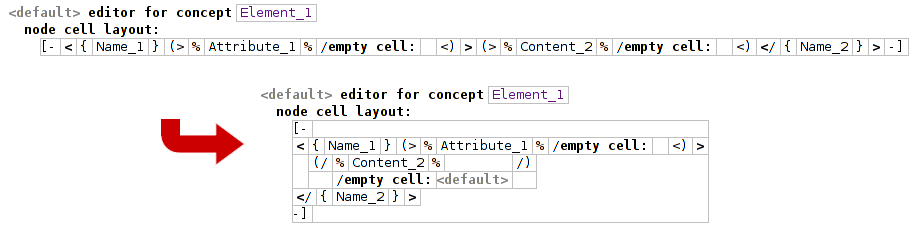
\includegraphics[scale=0.5]{./images/editor_adjustment.png}
	\caption{Projectional editor adjustment of the Element{\_}1 node}
	\label{fig:editor_adjustment}
\end{figure*}

In practice, however, the user still has to tweak the editor aspect --- to adjust the code layout --- because the heuristics are not 100\% reliable.
But it takes a very short time to reach optimal results (because MPS allows doing this very efficiently), as we show on the example of importing the JavaScript language~\cite{ref:javascript} and manually adjusting all editors that needed it, all that in a less than hour time.
More details are provided later in Section X (examples) --- there we describe this issue further.

\subsection{Text Generation}

The final/last, fourth step, is to create the TextGen aspect for each AST node.
The purpose of the TextGen aspect is to define, for a language element (AST node), what code in the BaseLanguage will be generated out of it, once we want to compile and run our MPS code/program.
This is needed to allow/enable users to generate plain-text source code representation out of the AST they built/created inside MPS.
Again, a TextGen aspect must be created for each language element.
Basically, it is a single method in the BaseLanguage (or in Java?) for each language element.
The method generates a string (plain-text) representation of the element, appends the string to the output stream, and then calls TextGen methods on all children of the element.

A very basic example of BaseLanguage code that can be used as the TextGen aspect of an \mpsconcept{Element{\_}1} node, which represents the full XML tag with content, is shown in Figure~\ref{fig:textgen_example}.
It appends all literals, properties, and children in the same order as they appear in the grammar definition.

\begin{figure}[ht]
	\centering
	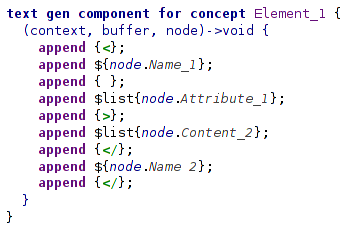
\includegraphics[width=90mm]{./images/textgen_example.png}
	\caption{Example of a~TextGen aspect}
	\label{fig:textgen_example}
\end{figure}

Like in the case of editor, we discovered some interesting challenges related to the code layout, whitespaces, and more (so on).
We describe our solution to the challenges here in this section.

The reader might have noticed that there is no whitespace handling inside of our SimpleXML grammar (Section XY, running example).
Grammars in the ANTLRv4 notation are usually written in such a manner that whitespace characters are skipped (ignored).
However/Nevertheless, TextGen aspect (generator) should/must know between which children there must be a whitespace and where it is forbidden (i.e., where to put some whitespace characters) so that the produced code is a valid one.
For example, in the case of the \antlrparserrule{element} rule, TextGen must determine that there should be a space in between \antlrparserrule{attribute} and \antlrlexerrule{Name}, while it is not required between \antlrliteral{\textless} and \antlrlexerrule{Name}.
In general, it is sufficient to put just a single space character at places/locations where there has to be some whitespace in order to make the code valid (syntactically correct).

Layout of the generated code is also important. For example, the user may want to produce more readable code by adding indentation or line breaks.

In fact, the problem of TextGen layout is quite similar to the one we have seen with the projectional editor, described in Section XY.
Since we are dealing mostly with text-based languages, their representation in projectional editor must be almost the same as their expected plain-text representation (output).
Therefore, one could use the same approach for editor and TextGen --- adding line breaks and indentation.
Once we would have some information about the layout for generating better projectional editor, we could leverage the same information and use it to improve TextGen.

Nevertheless, in our current approach, the editor aspects have to be adjusted manually, after the import is done, because for now it is the fastest and the most efficient way how to deal with the problem of customizing the editor to capture a nice layout.
Therefore, we used a different approach for TextGen --- a really simple heuristics which gives surprisingly good results.
In the first step, a very basic TextGen is created that inserts spaces in between every two tokens of the language element (AST node).
Then, as the second step, spaces are eliminated (restricted) from positions where they are not really needed.
We describe all the cases here:

\begin{enumerate}
	\item Whenever there is a non-alphabetical literal,	appearing as a plain string token defined in the grammar, that might get recognized by the parser safely without the need for a whitespace separator around, then we omit spaces around it.
		For example, consider \textbf{'\textless'} in SimpleXML.
	\item Another group are strings inserted by the user of the language, whose form is constrained by a regular expression.
		For example, an XML tag's name belongs to this group.
		They are usually values of properties defined in structure aspects.
		A space must be preserved only when a neighboring literal may end with an alphabetical character. Otherwise, we can omit the space.
		In practice, this will eliminate redundant spaces inside of quotes, next to semicolons, and around brackets, but, on the other hand, it will separate language keywords (function, var, in, etc.) from other content by keeping the space character in between them.
	\item Spaces are omitted also in the case of child nodes that are not present (e.g., when they are optional), and in the case of empty lists of child nodes, so that spaces do not accumulate.
	\item On the other hand, when two child elements are next to each other, we always insert space.
	\item Sequences of children are separated with space or with a line break.
\end{enumerate}
These few simple heuristics work surprisingly well and give us some very nice results.
We discuss our experience with XML, JSON, and JavaScript in Section XY (Evaluation).

Figure~\ref{fig:textgen_final} shows an example of a TextGen aspect for the full SimpleXML element.

\begin{figure}[ht]
	\centering
	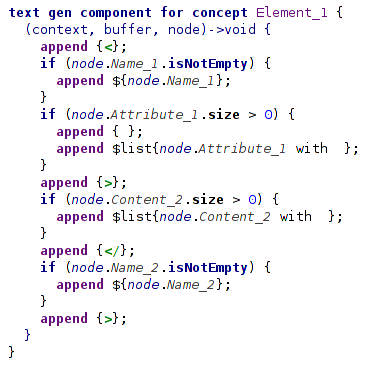
\includegraphics[width=95mm]{./images/textgen_final.png}
	\caption{Generated TextGen aspect for the SimpleXML element}
	\label{fig:textgen_final}
\end{figure}

The automatically generated TextGen code can be adjusted manually very easily, so that it generates nicely indented XML code.
In the case of the example above (in Figure F), we only need to wrap the \mpsconcept{Content{\_}2} child with indentation and change the sequence separator to a new line character.
The resulting adjusted aspect (code) is shown below in Figure~\ref{fig:textgen_adjusted}.

\begin{figure}[t!]
	\centering
	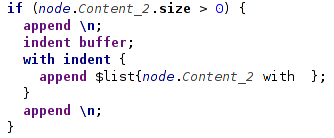
\includegraphics[width=85mm]{./images/textgen_adjusted.png}
	\caption{Adjusted indentation inside the TextGen aspect}
	\label{fig:textgen_adjusted}
\end{figure}

\subsection{Remarks about Grammars}

As we have already shown in previous sections, it is very easy to write a grammar in a way that will cause problems during import into MPS (or once it is imported).
Problems might occur during the creation of any aspect.
Here we will look at some general problems/issues that grammar import poses (might pose).
We will talk about these problems with respect to the challenges/obstacles we tried to overcome and which we described in previous sections (dedicated to structure, editor, and texgen, respectively).
We also show a few examples of additional possible complications.

\paragraph{Adjusting grammars.}
There are some cases, where altering the input grammar might yield far better MPS language.
We will show two examples how the usability of the resulting MPS language can be improved.
Let us look at the definition of an XML attribute in Figure~\ref{fig:xmlattribute}.

\begin{figure}[ht]
\centering
\begin{framed}
\begin{alltt}
	\antlrparserrule{attrib} : \antlrlexerrule{Name} \antlrliteral{=} \antlrlexerrule{STRING} ;
	\antlrlexerrule{STRING} : \antlrliteral{"} \antlrregex{~["]*} \antlrliteral{"}
	       | \antlrliteral{\textbackslash'} \antlrregex{~[']*} \antlrliteral{\textbackslash'} ;
\end{alltt}
\end{framed}
\caption{Definition of an XML attribute}
\label{fig:xmlattribute}
\end{figure}

The original XML grammar has quotes as a part of the value.
For the resulting MPS language, it would mean that there would be a placeholder for the attribute value that would expect us to input the leading and trailing quote together with the value too each time.
It would also be marked red (by the syntax checker) unless we enter both quotes inside the value since the regular expression checking for quotes will not match.
The user might be confused by this and will not be able to tell why his string value is incorrect.

In our SimpleXML language, we adjusted the grammar easily in the manner that we show in Figure~\ref{fig:xmladjustgrammar}.

\begin{figure}[ht]
\centering
\begin{framed}
\begin{alltt}
	\antlrparserrule{attrib} : \antlrlexerrule{Name} \antlrliteral{="} \antlrlexerrule{TEXT1} \antlrliteral{"}
	       | \antlrlexerrule{Name} \antlrliteral{=\textbackslash'} \antlrlexerrule{TEXT2} \antlrliteral{\textbackslash'} ;
	\antlrlexerrule{TEXT1} : \antlrregex{~["]*} ;
	\antlrlexerrule{TEXT2} : \antlrregex{~[']*} ;
\end{alltt}
\end{framed}
\caption{Adjusted grammar of SimpleXML}
\label{fig:xmladjustgrammar}
\end{figure}

We turned quotes into literals, thus ensuring that they will only appear in the projectional editor as fixed constant cells.
We will not have to encapsulate the value in them each time.
The user will only have to choose, which attribute version he wants to use (single or double quotes).

As the second example, we will use the ECMAScript\footnote{https://github.com/antlr/grammars-v4/blob/master/ecmascript/ECMAScript.g4} language otherwise known as JavaScript.
Every statement in JavaScript needs to be either followed by a semicolon, newline, file end or end of the block --- see the Figure~\ref{fig:javascriptstmt}.

\begin{figure*}[ht]
\centering
\begin{framed}
\begin{alltt}
	\antlrparserrule{eos} : \antlrlexerrule{SemiColon} | \antlrlexerrule{EOF} | {lineTerminatorAhead()}? 
	    | {{\_}input.LT(1).getType() == \antlrlexerrule{CloseBrace}}? ;
	\textcolor{gray}{// Example reference of the eos rule}
	\antlrparserrule{breakStmt} : \antlrlexerrule{Break} \antlrlexerrule{Identifier}? \antlrparserrule{eos} ;
\end{alltt}
\end{framed}
\caption{Statements in JavaScript}
\label{fig:javascriptstmt}
\end{figure*}

Because there are multiple options, our import plugin would create a placeholder at the end of every statement.
Every language element representing a statement would have one child of the \mpsinterface{IEos} interface type.
This placeholder needs to be manually filled in for each statement.

Since the projectional editor has much bigger power over the form of the code, we (a user) might want to have each statement on a separate line.
Since we can differentiate between statements on the AST level, we do not need an explicit separator between them.
This means that we might want to simplify the language and leave the semicolon out, or leave it just as a constant fixed part of the projectional editor, but not as something the user must explicitly fill in.
Then we can just put each statement on a separate line as it is usual for JavaScript code, but we do not need the semicolon anymore.
This small adjustment is very quick when done inside the grammar.
We just change the \antlrparserrule{eos} rule to the form shown in Figure~\ref{fig:eosrule}.

\begin{figure}[ht]
\centering
\begin{framed}
\begin{alltt}
	\antlrparserrule{eos} : \antlrliteral{;} ;
\end{alltt}
\end{framed}
\caption{eos parser rule}
\label{fig:eosrule}
\end{figure}

This way, we can change the grammar in a way that it will not describe the same ECMAScript language as before, but will definitely make our MPS language more usable.
TextGen aspect may be defined in such a way that puts the semicolon back (after each statement) in the generated plain-text representation.
This would be very important especially when JavaScript is available as another base language (which is actually a plan (future work) of the JetBrains company).

Above, we have shown that adjusting the input grammar might be a very fast mean of tweaking/improving the usability of generated MPS language, and sometimes it may be the only proper solution in some complex situations.
In general, the question we can ask ourselves is whether one aims for a full precise/faithful port of the input language or for an MPS alternative.

\todo{Nahradit slovo "break" v nasledujicich odstavcich (v kontextu "break the parser") za vhodnejsi slovo ktere pusobi vic odborne.}

\paragraph{Breaking grammars and parsers.}
However, we have found that there is one big problem with grammar adjustment that we would like to point out.
The problem is that it is very easy to change the input ANTLR grammar in a way that breaks the ANTLR parser generated out of it.
By breaking we mean that it stops parsing the original language.
We illustrate the problem on our SimpleXML language.

As stated before, when creating the SimpleXML grammar, we have started off with the original XML grammar\footnote{https://github.com/antlr/grammars-v4/tree/master/xml} and did some adjustments to it.
We ended up with a grammar that can be processed by our method/plugin and creates a nice usable MPS language.
Nevertheless, we noticed that even though the imported language behaves well enough and mimics the XML language quite nicely, the ANTLR parser generated out of this grammar no longer parses XML successfully.
Some changes we have made, such as the attribute adjustment, broke the grammar down.
More precisely, our changes improved the MPS language while breaking down the parser, and we have not even noticed it because, from the perspective of MPS, the imported language still corresponds to XML.

What we are trying to say (show here) is that it is very easy to perform a grammar adjustment that will, at first, seem harmless and valid inside MPS, but will break the parser.
The problem is that the user performing this change probably will not be aware of breaking it.

The main (underlying) cause of this problem is the way the ANTLR parser is implemented and the quite different purpose we are using the grammar for in our project/tool/method.
There are many ways how various parsers deal with, for example, token matching.
For instance, ANTLR introduces so called \emph{greedy} and \emph{non-greedy} operators.
The greedy way, in which ANTLR matches input on defined tokens and prioritizes their selection, makes some rules very dangerous.
When a rule matches a wide range of input, it might happen during parsing that it is prioritized over other rules and swallows a lot more input than the author of it intended.
Usually, these dangerous rules are bound to some parser context, which makes them behave well.

However, for practical reasons, it is very important that grammar is not broken by our custom adjustments (and that the ANTLR parser of the language works properly), because we might need to automatically generate parsers of the adjusted language.
Imagine this very real scenario (that will be supported in the future):
\begin{enumerate}
	\item We have imported the language inside MPS.
	\item MPS now knows the structure of the language, and we can code in MPS using this language.
	\item We would expect MPS to be able to load an existing source code, written in this language, from a text file and import it inside MPS.
	\item We would like to use MPS to safely edit this code, using all the features of MPS.
	\item We would also like to export the code in a plain-text form again and save it back to the source file.
\end{enumerate}
In order to make this happen, we must be able to generate a correctly-working ANTLR parser out of the adjusted source grammar that we used to (that helped us) import the language.
We must also be able to match nodes of the AST coming out of the ANTLR parser to elements of the MPS language, and we must build the MPS AST out of the ANTLR AST.
